\documentclass[]{report}
\usepackage{mathtools}
\usepackage{amsmath}
\usepackage{amssymb}    % Math symbols such as \mathbb
\usepackage{amsthm}
\usepackage[utf8]{inputenc}
\usepackage{graphicx}
\usepackage{syntax}
%\usepackage{synttree}
\usepackage{tikz}
\usepackage{tikz-qtree}
\usetikzlibrary{positioning,shapes.geometric}
\usepackage{listings}
\usepackage{natbib}
\usepackage{algorithmicx}
\usepackage{algpseudocode}
\usepackage{soul}
\usepackage{droidmono}
\usepackage[hidelinks]{hyperref}
\sethlcolor{gray}


\lstdefinestyle{complex}
{	
	language=scala,
	numbers=left,
	tabsize=2,
	numbersep=0.5pt
}

\lstdefinestyle{simple111}
{
	basicstyle=\scriptsize\fdmfamily,
	language=scala,
	tabsize=2
}

% thanks to https://tex.stackexchange.com/a/202517
\lstdefinestyle{simple}{
	basicstyle=\scriptsize\fdmfamily,
	frame=tb,
	language=scala,
	aboveskip=3mm,
	belowskip=3mm,
	showstringspaces=false,
	columns=flexible,
	basicstyle={\small\ttfamily},
	numbers=none,
	numberstyle=\tiny\color{gray},
	keywordstyle=\color{blue},
	commentstyle=\color{dkgreen},
	stringstyle=\color{mauve},
	%frame=single,
	breaklines=true,
	breakatwhitespace=true,
	tabsize=3,
}


% thanks to https://tex.stackexchange.com/a/53359
\algnewcommand\algorithmicassert{\textbf{assert }}
\algnewcommand\Assert[1]{\State \algorithmicassert #1}%



%https://tex.stackexchange.com/questions/9057/best-practice-for-control-flow-charts

\newcommand{\motexample}{
		\begin{figure}[!h]
		\begin{center}
		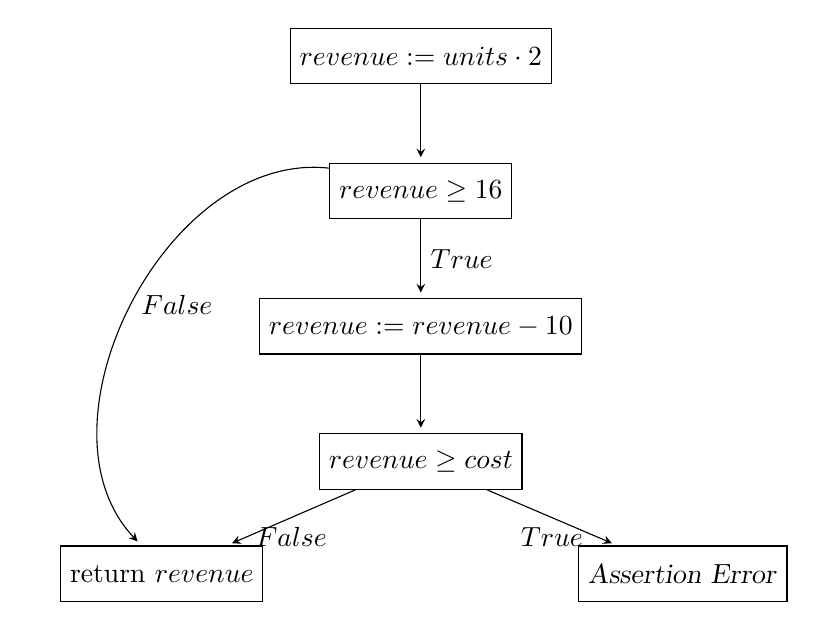
\begin{tikzpicture}[%
		->,
		shorten >=2pt,
		>=stealth,
		node distance=1cm,
		noname/.style={%
			minimum width=4em,
			minimum height=2em,
			draw,
			align=left
		}
		]
		\node[noname] (1)                                             {$revenue := units \cdot 2$};
		\node[noname] (2) [below=of 1]                                {$ revenue \geq 16$};
		\node[noname] (3) [below=of 2]						  {$revenue := revenue - 10$};
		\node[noname] (4) [below= of 3]							      {$ revenue \geq cost$};
		\node[noname] (5) [below right= of 4]						  {\textsl{Assertion Error}};
		\node[noname] (6) [below left= of 4]						  {return $revenue$};
		
		
		\path (1) edge             									node {} (2)
		(2) edge [bend right=70pt] 							node[right] {$False$} (6)
		(2) edge 											node[right] {$True$} (3)
		(3) edge											node {} (4)
		(4) edge 											node[right, below] {$True$} (5)
		(4) edge											node[right, below] {$False$} (6);
		\end{tikzpicture}
	\end{center}
	\caption{Control-flow graph for \textsc{ComputeRevenue}}
	\end{figure}
}

\newcommand{\sumprogram}{
	\begin{figure}[!h]
	\begin{center}
		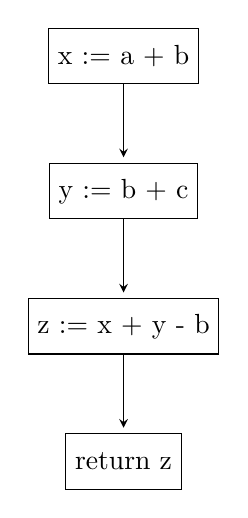
\begin{tikzpicture}[%
		->,
		shorten >=2pt,
		>=stealth,
		node distance=1cm,
		noname/.style={%
			minimum width=4em,
			minimum height=2em,
			draw
		}
		]
		\node[noname] (1)                                             {x := a + b};
		\node[noname] (2) [below=of 1]                                {y := b + c};
		\node[noname] (3) [below=of 2] 								  {z := x + y - b};
		\node[noname] (4) [below=of 3]                                {return z};
		
		\path (1) edge                   node {} (2)
		(2) edge                   node {} (3)
		(3) edge                   node {} (4);
		\end{tikzpicture}
	\end{center}
	\caption{Control-flow graph for ComputeSum}
	\end{figure}
}

\newcommand{\pow}{
	\begin{figure}[!h]
	\begin{center}
		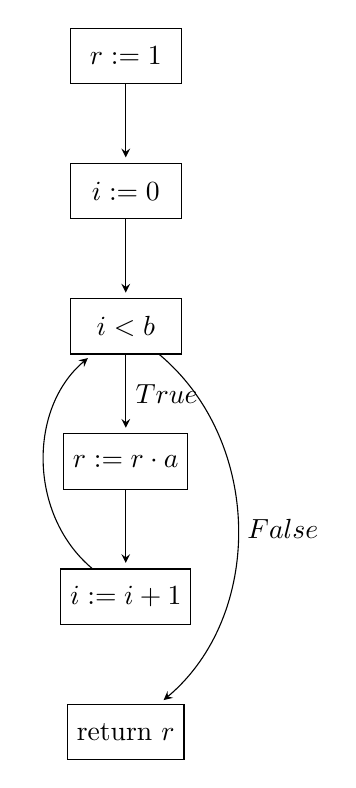
\begin{tikzpicture}[%
		->,
		shorten >=2pt,
		>=stealth,
		node distance=1cm,
		noname/.style={%
			minimum width=4em,
			minimum height=2em,
			draw
		}
		]
		\node[noname] (1)                                             {$r := 1$};
		\node[noname] (2) [below=of 1]                                {$i := 0$};
		\node[noname] (3) [below=of 2] 								  {$i < b$};
		\node[noname] (4) [below=of 3]								  {$r := r\cdot a$};
		\node[noname] (5) [below=of 4]								  {$i := i + 1$};
		\node[noname] (6) [below=of 5]								  {return $r$};
		
		
		\path (1) edge             									node {} (2)
		(2) edge                  								    node {} (3)
		(3) edge [bend left = 50pt] 								node[right] {$False$} (6)
		(3) edge                 								    node[right] {$True$} (4)
		(4) edge 												    node {} (5)
		(5) edge [bend left = 50pt]								node {} (3);
		\end{tikzpicture}
	\end{center}
	\caption{Control-flow graph for \textsc{ComputePow}}
	\end{figure}
}

\newcommand{\ifstm}{
	\begin{figure}[!h]
		\begin{center}
			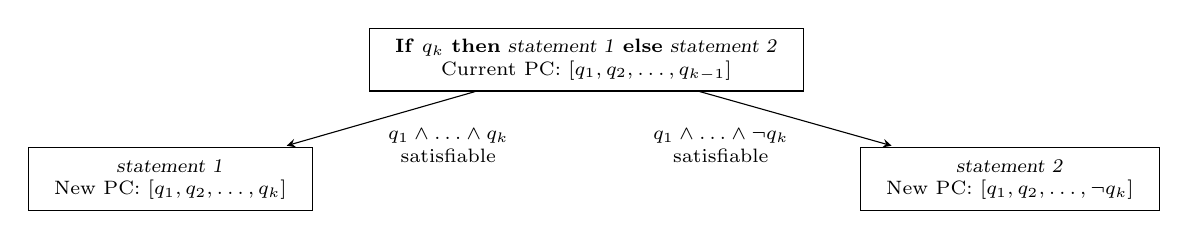
\begin{tikzpicture}[%
			font=\scriptsize,
			->,
			shorten >=2pt,
			>=stealth,
			node distance=1cm,
			noname/.style={%
				minimum width=4em,
				minimum height=2em,
				draw
			}
			]
			\node[noname] (1)    {\begin{tabular}{c}
				\textbf{If} $q_k$ \textbf{then} \textsl{statement 1} \textbf{else} \textsl{statement 2}\\
				Current PC: $[q_1, q_2, \ldots, q_{k-1}]$
				\end{tabular}};
			\node[noname] (2) [below left= of 1] {\begin{tabular}{c}
				\textsl{statement 1}\\
				New PC: $[q_1, q_2, \ldots, q_k]$
				\end{tabular}};
			\node[noname] (3) [below right= of 1] {\begin{tabular}{c}
				\textsl{statement 2}\\
				New PC: $[q_1, q_2, \ldots, \neg q_k]$
				\end{tabular}};
			
			\path (1) edge node[below right, align=center] {$q_1\land\ldots \land q_k$ \\ satisfiable} (2) 
			(1) edge node[below left, align=center] {$q_1\land \ldots \land \neg q_k$\\satisfiable} (3);	
 			\end{tikzpicture}
		\end{center}
		\caption{Abstract overview of the symbolic execution of an \textsl{if}-statement, which potentially leads to two new execution paths, each with a new \pc.}
	\end{figure}
}
\newcommand{\exectree}{
	\begin{figure}[!h]
		\begin{center}
			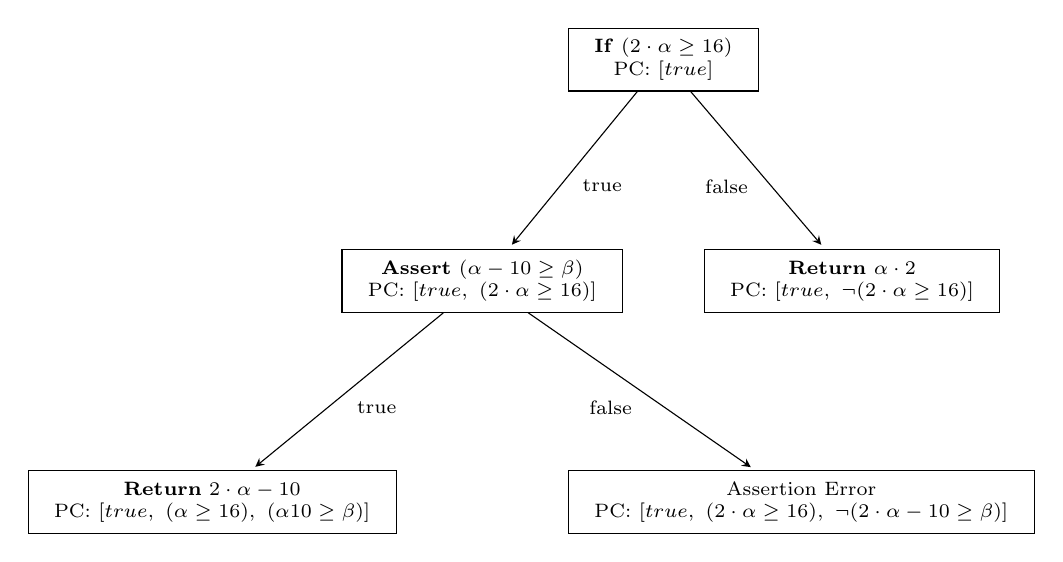
\begin{tikzpicture}[%
			align = center,
			font=\scriptsize,
			->,
			shorten >=2pt,
			>=stealth,
			node distance=2cm and -0.7cm,
			noname/.style={%
				minimum width=4em,
				minimum height=2em,
				draw
			}
			]
			\node[noname] (1)  {\begin{tabular}{c}
				\textbf{If} $(2\cdot \alpha \geq 16)$\\
				PC: $[true]$
				\end{tabular}};
			\node[noname] (2) [below left= of 1] {\begin{tabular}{c}
				\textbf{Assert} $(\alpha - 10 \geq \beta)$\\
				PC: $[true, \ (2\cdot\alpha \geq 16)]$
				\end{tabular}};
			\node[noname] (3) [below right= of 1] {\begin{tabular}{c}
					\textbf{Return} $\alpha \cdot 2$\\
					PC: $[true, \ \neg(2 \cdot\alpha \geq 16)]$
				\end{tabular}};
			\node[noname] (4) [below left = of 2] {\begin{tabular}{c}
				\textbf{Return} $2\cdot \alpha - 10$\\
				PC: $[true, \  (\alpha \geq 16), \ (\alpha  10 \geq \beta)]$
				\end{tabular}};
			\node[noname] (5) [below right = of 2] {\begin{tabular}{c}
				Assertion Error\\
				PC: $[true, \ (2\cdot \alpha \geq 16), \ \neg(2\cdot \alpha - 10 \geq \beta)]$
				\end{tabular}};
			
			\path (1) edge node[below right] {true} (2)
			(1) edge node[below left] {false} (3)
			(2) edge node [below right] {true} (4)
			(2) edge node [below left] {false} (5);
			\end{tikzpicture}
		\end{center}
	\end{figure}

}

\graphicspath{ {images/} }


\newcommand{\explanguage}{\textsl{SIMPL }}
\newcommand{\pc}{\emph{path-constraint} }
\newcommand{\alt}{ \ | \ }
% Title Page
\title{
	\textbf{Symbolic \& Concolic Execution}\\
	{ Symbolsk og Concolic eksekvering}\\
	\bigskip
	%{
\includegraphics[scale=0.5]{ausegl_blaa.png}}	
	\large Bachelor report (15 ECTS) in Computer Science, Aarhus University\\
	}
\author{Søren Baadsgaard $\cdot$ 201305284 \\
	Advisor: Magnus Madsen}
\begin{document}
\maketitle

\begin{abstract}
	The focus of this report is symbolic execution, which is a technique for systematically exploring all execution paths of a program, and for each path generate concrete input values that will execute along this path. We describe the theory behind symbolic execution and discuss a number of limitations to the technique. Furthermore we describe a different technique called concolic execution, that combines concrete and symbolic execution to mitigate some of the challenges of pure symbolic execution. Finally, we demonstrate symbolic execution by describing and comparing an implementation of both a concrete and symbolic interpreter for a small toy language. 
\end{abstract}

\tableofcontents

\chapter{Introduction}
	Proper testing of programs requires a good selection of input values that cover all edge cases of the program to ensure that it behaves as expected. Choosing such a selection is often a difficult and time consuming task, and so we risk ending up with a lackluster choice of test cases, which leaves large parts of the program untested. The goal of this report is to study \emph{symbolic} execution, which is a classical technique to systematically explore all execution paths of a program and generate concrete input values that will follow these execution paths and thereby obtain test cases that properly cover the entire program. To this, the program is executed symbolically by replacing the input values with symbolic values that represents arbitrary concrete values. Whenever a conditional statement is executed, there are two potential execution paths to follow. If both paths are feasible, the execution splits into two executions, each following a different path. Each execution keeps track of the constraints that the input values must satisfy to follow that path, and from these constraints we can derive concrete input values that will execute along the same path.
\\ 
We will also study a modern approach called \emph{concolic} execution that combines concrete and symbolic execution. In this technique, the program is executed with initially random concrete input values. During the execution, we maintain both symbolic and concrete values for all variables, and whenever the execution branches, the choice of branch is registered in a list of constraints, using the symbolic values. At the end of the execution, this list of constraints is used to generate a new set of concrete input values that will cause the program to execute along a different path. This process is repeated until all execution paths have been explored.
 

\newpage In chapter 2 we give a motivating example, to illustrate the usefulness of symbolic execution. In chapter 3 we will describe the principles of classical symbolic execution.  
 We will also study some key challenges and limitations to this technique. 
 In chapter 4 we will describe the principles of concolic execution. We will also be comparing the two techniques to see what advantages concolic execution offer over classical symbolic execution. Finally, in chapter 5 and 6 we demonstrate the principles of symbolic execution by implementing a concrete and a symbolic interpreter for a small toy language.  
	
\chapter{Motivation}
	In this chapter we will present the motivation for this project, by considering a motivating example that illustrates the usefulness of symbolic execution as a software testing technique.

\section{A motivating example}
Consider a company that sells a product with a unit price 2. If the revenue of an order is greater than or equal 16, a discount of 10 is applied. The following program that takes integer inputs $units$ and $cost$ computes the total revenue based on this pricing scheme. 


\begin{figure}[!h]
	\begin{algorithmic}[1]
		\Procedure{ComputeRevenue}{$units, cost$}
		\State $revenue := 2\cdot units$
		\If{$revenue \geq 16$}
		\State $revenue := revenue - 10$
		\Assert{$revenue \geq cost$}
		\EndIf
		\State \Return{$revenue$}
		\EndProcedure
	\end{algorithmic}
\end{figure}

\motexample

\newpage

After applying the discount, we assert that $revenue \geq cost$ since we do not wish to sell at a loss. 
We would like to know if this program ever fails due an assertion error, so we have to figure out if there exist integer inputs for which the program reaches the \textsl{Assertion Error} node in the control-flow graph. 
We might try to run the program on different input values, e.g $(units = 8, cost = 5)$, $(units = 7, cost = 10)$. These input values does not cause the program to fail, but we are still not convinced that it wont fail for some other input values.
By observing the program for some time, we realize that the input must satisfy the following two constraints to fail:

\begin{align*}
	 units \cdot 2 & \geq 16\\
	 units \cdot 2 & < cost
\end{align*}

which is the case e.g for $(units = 8, cost = 7)$. This realization was not immediately obvious, and for more complex programs, answering the same question is even more difficult. The key insight is that the conditional statements dictates which execution path the program will follow. In this report we will present \emph{symbolic execution}, which is a technique to systematically explore different execution paths and generate concrete input values that will follow these same paths. 
\chapter{Principles of symbolic execution}
	In this chapter we will cover the theory behind symbolic execution. We will start by describing what it means to \emph{symbolically} execute a program and how we deal branching. We will also explain the connection between a symbolic execution of a program, and a concrete execution. We shall restrict our focus to programs that takes integer values as input and allows us to do arithmetic operations on such values. In the end we will cover the challenges and limitations of symbolic execution that arises when these restrictions are lifted. 


\section{Symbolic executing of a program}
	
	During a normal execution of a program, input values consists of integers. During a symbolic execution we replace concrete values by symbols e.g $\alpha$ and $ \beta$, that acts as placeholders for actual integers. We will refer to symbols and arithmetic expressions over these as \emph{symbolic values}.
	 The program environment consists of variables that can reference both concrete and symbolic values. \cite{CadarSen13} \cite{King76}.
	\\
	To illustrate this, we consider the following program that takes parameters $a, b$ and $ c$ and computes their sum. The computation may seem unnecessarily complicated, but we do it this way to clearly what we mean by symbolic values, and how they relate to concrete values.
	\begin{figure}[!h]
		\begin{algorithmic}
			\Procedure{ComputeSum}{$a, b, c$}
			\State $ x := a + b$
			\State $ y := b + c$
			\State $ z := x + y - b$
			\State \Return{$z$}
			\EndProcedure
		\end{algorithmic}
	\end{figure}

	\sumprogram{}
	\newpage
	Lets consider running the program with concrete values $a = 2, b = 3$ and $c = 4$. We then get the following execution:
	First we assign $a+b = 5$ to the variable $x$. Then we assign $b + c = 7$ to the variable $y$. Next we assign $x + y - b = 9$ to variable $z$ and finally we return $z = 9$, which is indeed the sum of 2, 3 and 4. 
	\\
	Let us now run the program with symbolic input values $\alpha, \beta$ and $\gamma$ for $a, b$ and $c$ respectively. 

	
	We then get the following execution: First we assign $\alpha + \beta$ to $x$. We then assign $\beta + \gamma$ to $y$. Next we assign $(\alpha + \beta) + (\beta + \gamma) - \beta$ to $z$.Finally we return $z = \alpha + \beta + \gamma$. We can conclude that the program correctly computes the sum of $a, b$ and $c$, for any possible value of these.
	
\section{Execution paths and path constraints}
		The program that we considered in the previous section contains no conditional statements, which means it only has a single possible execution path. In general, a program with conditional statements $s_1, s_2, \ldots, s_n$ with conditions $q_1, q_2, \ldots, q_n$, will have several execution paths that are uniquely determined by the value of these conditions. In symbolic execution, we model this by introducing a \emph{path-constraint} for each execution path. The \emph{path-constraint} is a list of boolean expressions $\lbrack q_1, q_2, \ldots, q_k \rbrack$ over the symbolic values, corresponding to conditions from the conditional statements along the path. At the start of an execution, the \emph{path-constraint} only contains the expression $true$, since we have not encountered any conditional statements. to continue execution along a path, $q_1 \land \ldots \land q_k$ must be \emph{satisfiable}. To be \emph{satisfiable}, there must exist an assignment of integers to the symbols, such that the conjunction of the conditions evaluates to true. For example, $q = (2\cdot \alpha > \beta) \land (\alpha < \beta)$ is satisfiable, because we can choose $\alpha = 10$ and $\beta = 15$ in which case $q$ evaluates to \emph{true}. On the other hand $q' = (2 \cdot \alpha < 4) \land (\alpha > 4)$ is clearly not satisfiable since the first condition stipulates that $\alpha < 2$ and the second condition stipulates that $\alpha > 4$.
		\\
		
		\iffalse
		 This situation can for example occur if we are executing two consecutive \textsl{if}-statements, where the first one has condition $2\cdot \alpha < 4$ and the second has condition $\alpha > 4$. 
		\fi
	
		\noindent Whenever we reach a conditional statement with condition $q_k$, we consider the two following expressions:
	
		\begin{enumerate}
			\item $ q_1 \land q_2 \land \ldots \land q_k$
			\item $ q_2 \land q_2 \land \ldots \neg q_k$
		\end{enumerate}	
		This gives a number of possible scenarios:	
		\ifstm	
		\begin{itemize}
			\item \textbf{Only the first expression is satisfiable}: Execution continues with a new \emph{path-constraint} $\lbrack q_1, q_2, \ldots, q_k \rbrack$, along the path corresponding to $q_k$ evaluating to to \emph{true}.
			\item \textbf{Only the second expression is satisfiable}:  Execution continues with a new \emph{path-constraint} $\lbrack q_1, q_2, \ldots, \neg q_k \rbrack$, along the path corresponding to $q_k$ evaluating to to \emph{false}.
			
			\item \textbf{Both expressions are satisfiable}: In this case, the execution can continue along two paths; one corresponding to the condition being \emph{false} and one being \emph{true}. At this point we \emph{fork} the execution by considering two different executions of the remaining part of the program. Both executions start with the same environment and \emph{path-constraints} that are equal up to the final condition. One will have $q_k$ as the final condition and the other will have $\neg q_k$. 
			These two executions will continue along different execution paths that differ from this conditional statement and onward \cite{King76}.
		\end{itemize} 
		
		To illustrate this, we consider the program from the motivating example, that takes input parameters $units$ and $costs$:
		
		\motexample{}
		\newpage
		We assign symbolic values $\alpha$ and $\beta$ to $units$ and $cost$ respectively, and get the following symbolic execution:
		
		First we assign $2\cdot \alpha$ to $revenue$. We then reach an \textsl{if}-statement with condition $\alpha \cdot 2 \geq 16$. To proceed, we need to check the satisfiability of the following two expressions:
		\begin{enumerate}
			\item $true \land (\alpha \cdot 2 \geq 16)$
			\item $true \land \neg (\alpha \cdot 2 \geq 16)$.
		\end{enumerate}
		Since both these expressions are satisfiable, we need to fork. We continue execution with a new  \emph{path-constraint} $\lbrack true, (\alpha \cdot 2 \geq 16) \rbrack$, along the path corresponding to the condition evaluating to \emph{true}. We also start a new execution with the same environment and a \emph{path-constraint} equal to $\lbrack true, \neg (\alpha \cdot 2 \geq 16) \rbrack$. This execution will continue along the path corresponding to the condition evaluating to \emph{false}, and it immediately reaches the return statement and returns $\alpha \cdot 2$.
		The first execution assigns $2\cdot \alpha - 10$ to $revenue$ and then reach an \textsl{assert}-statement with condition $2\cdot \alpha - 10 \geq \beta$. We consider the following expressions:
		\begin{enumerate}
			\item $true \land (\alpha \cdot 2 \geq 16) \land (((2\cdot \alpha) - 10) \geq \beta)$
			\item $true \land (\alpha \cdot 2 \geq 16) \land \neg (((2\cdot \alpha) - 10) \geq \beta)$
		\end{enumerate}
		Both of these expressions are satisfiable, so we fork again. In the end we have discovered all three possible execution paths with the following \emph{path-constraints}:
		\begin{enumerate}
			\item $true \land \neg (\alpha \cdot 2 \geq 16)$
			\item $true \land (\alpha \cdot 2 \geq 16) \land (((2\cdot \alpha) - 10) \geq \beta)$
			\item $true \land (\alpha \cdot 2 \geq 16) 
			\land \neg (((2\cdot \alpha) - 10) \geq \beta)$.
		\end{enumerate}
		
		%\exectree
		The first two \emph{path-constraints} corresponds to the two different paths that leads to the return  ment, where the first one returns $2\cdot \alpha$ and the second one returns $2\cdot \alpha - 10$. Inputs that satisfy these, does not result in a crash.
		The final \emph{path-constraint} corresponds to the path that leads to the \textsl{Assertion Error}, so we can conclude that all input values that satisfy these constraints, will result in a program crash.
	
		
\section{Constraint solving}
	As we just described, a symbolic execution of a program results in one or more \emph{path-constraints} corresponding to each possible execution path. We know that each of these \emph{path-constraints} are satisfiable, so we can solve the \pc by finding an assignment of concrete values to the symbols, that causes it to evaluate to true. Consider for example 
	
	\begin{equation*}
		true \land (\alpha \cdot 2 \geq 16) \land (2\cdot \alpha - 10 \geq \beta)
	\end{equation*}
	
	which is one of the three resulting \emph{path-constraints} from the motivating example. From the first condition we get that $\alpha \geq 8$, so we can choose $\alpha = 8$. The second condition then gives us that $6 \geq \beta$, so we can choose $\beta = 6$. If we do a concrete execution of the program with $units = 8$ and $cost = 6$, it will follow the execution path that correspond to this \pc. We can do the same for the remaining two \emph{path-constraints}, and in the end we will have a pair of concrete input values for each possible execution path. So symbolic execution not only allows us to explore all possible execution paths, it also allows to generate a small set of concrete input values that cover all these paths.  

	
	\iffalse
	In the previous section we described how to handle programs with multiple execution paths by introducing a \emph{path-constraint} for each path, which a list of constraints on the input symbols. This system of constraints defines a class of integers that will cause the program to execute along this path. By solving the system from each \emph{path-constraint}, we obtain a member from each of class which forms a set of concrete inputs that cover all possible paths.    
	
	If we consider the motivating example again, we found three different paths, represented by the following \emph{path-constraints}:
	\begin{enumerate}
		\item $true \land \neg (\alpha \cdot 2 \geq 16)$
		\item $true \land (\alpha \cdot 2 \geq 16) \land (2\cdot \alpha - 10 \geq \beta)$
		\item $true \land (\alpha \cdot 2 \geq 16) \land \neg (2\cdot \alpha - 10 \geq \beta)$.
	\end{enumerate}
	
	By solving for $\alpha$ and $\beta$, we obtain the set of inputs $\{(7, \beta), (8,6), (8, 7)\}$, that covers all possible execution paths. Note that we have excluded a concrete value for $\beta$ in the first test case, because the \emph{path-constraint} does not depend on the value of $\beta$. 
	 
	\fi 
\section{Limitations and challenges of symbolic execution}
	So far we have only considered symbolic execution of programs with a small number of execution paths. Furthermore, the constraints placed on the input symbols have all been linear expressions.
	In this section we will cover the challenges that arise when we consider more general programs.
	
	\subsection{The number of possible execution paths} 
		Since each conditional statement in a given program can result in two different execution paths, the total number of paths to be explored is potentially exponential in the number of conditional statements. 
		For this reason, the running time of the symbolic execution quickly gets out of hands if we explore all paths. 
		 The challenge gets even greater if the program contains a looping statement. In this case, the number of execution paths is potentially infinite \cite{CadarSen13}.
		  We illustrate this by considering the following program that computes $a^b$ for integers $a$ and $b$, with symbolic values $\alpha$ and $\beta$ for $a$ and $b$:
		\begin{figure}[!h]
			\begin{algorithmic}
				\Procedure{ComputePow}{$a,b$}
				\State $r := 1$
				\State $i := 1$
				\While{$i \leq b$}
					\State $ r := r\cdot a$
					\State $ i := i + 1$
				\EndWhile
				\State \Return{$r$}
				\EndProcedure
			\end{algorithmic}
		\end{figure}
		\pow{}
		
	This program contains a \textsl{while}-statement with condition $i \leq b$. The $k'th$ time we reach this statement we will consider the following two expressions:
	\begin{enumerate}
		\item $true \land (1 \leq \beta) \land (2 \leq \beta) \land \ldots \land (k-1 \leq \beta) $
		\item $true \land (1 \leq \beta) \land (1 \leq \beta) \land \ldots \land \neg (k-1 \leq \beta) $.
	\end{enumerate}
	Both of these expressions are satisfiable, so we fork the execution. This is the case for any $k > 0$, which means that the number of possible execution paths is infinite. If we insist on exploring all paths, the symbolic execution will simply continue for ever. To avoid this, we can include some other termination criteria. As an example, we could have limit on the number of times we allow the execution to fork, and as soon as this limit is reached we simply ignore any further execution paths.
	
	\subsection{Deciding satisfiability of \emph{path-constraints}}
	A key component of symbolic execution, is deciding if a \emph{path-constraint} is satisfiable, in which case the corresponding execution path is eligible for exploration. Consider the following \emph{path-constraint} from the motivating example:
	
	\begin{equation*}	
		true \land (\alpha \cdot 2 \geq 16) \land \neg (2\cdot \alpha - 10 < \beta).
	\end{equation*}
	
	To decide if this is satisfiable or not, we must determine if there exist an assignment of integer values to $\alpha$ and $\beta$ such that the formula evaluates to \emph{true}. We notice that the formula is a conjunction of linear inequalities. We can assign these to variables $q_1$ and $q_2$ and get
	\begin{align*}
		q_1 & = (\alpha \cdot 2 \geq 16) \\
		q_2 & = (2\cdot \alpha - 10 < \beta)
	\end{align*}
	The formula would then be $true\land q_1 \land \neg q_2$,
	where $q_1$ and $q_2$ can have values \emph{true} or \emph{false} depending on whether or not the linear inequality holds for some integer values of $\alpha$ and $\beta$. The question then becomes twofold: Does there exist an assignment of \emph{true} and \emph{false} to $q_1$ and $q_2$ such that the formula evaluates to true? And if so, does this assignment lead to a system of linear inequalities that is satisfiable?
	In this example, we can assign \emph{true} to $q_1$ and \emph{false} to $q_2$, which gives the following system of linear inequalities:
	\begin{align*}
		& \alpha \cdot 2 \geq 16 \\
		2  \cdot & \alpha - \beta \geq 10 
	\end{align*}
	
	where we gathered the constant terms on the left hand side, and the symbols the right hand side. From the first equation we get that $\alpha \geq 8$ so we choose $\alpha = 8$. From the second equation we then get that $\beta \leq 6$, so we choose $\beta = 6$ and this gives us a satisfying assignment for the path constraint. Since deciding satsifiability of a \pc is such an critical part of symbolic execution, it is important to know if we can always correctly \emph{yes} or \emph{no}. In the next section we will study this question more closely, and we will see that it depends on what sort of constraints we place on the input values. 
	\subsubsection{The SMT problem}

	The example we just gave, is an instance of the \emph{Satisfiability Modulo Theories}(SMT) problem. To understand SMT, we first consider the \emph{Boolean Satisfiability}(SAT) problem. In this problem we are given a logical formula over boolean variables $q_1, q_2, \ldots, q_n$. We want to decide if there exists an assignment of truth values to each variable such that the formula evaluates to true. for example, $(q_1 \land \neg q_2)$ is a \emph{yes}-instance of this problem, since $q_1 = true$ and $q_2 = false$ causes the formula to evaluate to \emph{true}. On the other hand $q_1 \land q_2 \land \neg q_2$ is a \emph{no}-instance since the formula is clearly false no matter which values we assign. This problem is \emph{decidable}, meaning that we can always correctly answer \emph{yes} or \emph{no} to whether or not a given formula is satisfiable. However it is also NP-complete, which means that the best known method for solving this problem takes worst-case exponential time. SMT is then an extention of this problem. We now let the boolean variables $q_1, q_2, \ldots, q_n$ represent expressions from some theory such as the \emph{theory of integer linear arithmetic(LIA)} \cite{DeMoura2011}. In LIA, an expression e is defined as 
		\begin{alignat*}{3}
			e & \in \textsc{Expression} && := \quad p \bowtie p\\
			\bowtie & \in \textsc{Constraint} && := \quad \leq \alt \geq \alt =\\
			p & \in \textsc{Polynomial} && := \quad a \alt a\cdot x \alt p \circ p\\
			\circ & \in \textsc{Operator} && := \quad + \alt - \\
			a & \in \textsc{Integer} && := \quad 0 \alt 1 \alt -1 \alt \ldots\\ 
			x & \in \textsc{Variable} && := \quad a \alt b \alt c \alt \ldots		
		\end{alignat*} 
	We now want to decide if the formula is satisfiable with respect to the theory. To be satisfiable w.r.t LIA, we require that there exist an assignment of truth values to the boolean variables such that the formula evaluates to \emph{true}, and that for such an assignment, there exists an assignment of integer values to the variables in the underlying expressions such that all the constraints are satisfied. In the previous section we showed that 
	
	\begin{equation*}	
	true \land (\alpha \cdot 2 \geq 16) \land \neg (2\cdot \alpha - 10 < \beta).
	\end{equation*}

	is a \emph{yes}-instance of the SMT problem, since we could let $q_1$ represent $(\alpha \cdot 2 \geq 16)$ and $q_2$ represent $(2\cdot \alpha - 10 < \beta)$. We could then assign $q_1 = true$ and $q_2 = false$. For this assignment of truth variables, we could choose $\alpha = 8$ and $\beta = 6$ in which case all the constraints hold. On the other hand 
	
	\begin{equation*}
		(2\cdot \alpha < 4) \land (\alpha > 4)
	\end{equation*}
	
	is clearly a \emph{no}-instance. If we let $q_1$ represent $(2\cdot \alpha < 4)$ and $q_2$ represent $(\alpha > 4)$, the formula becomes $q_1\land q_2$. The only assignment of truth variables that satisfy this is $q_1 = true$ and $q_2 = true$. But it is clear that there does not exist an integer value for $\alpha$ such that both the constraints hold. LIA is a \emph{decidable} theory, meaning that we can always correctly answer \emph{yes} or \emph{no} to an instance of the SMT problem, when it is with respect to LIA. Given an SMT formula, we can construct an Integer Linear Program with the expressions from the formula as constraints. This program will we feasible if and only if the SMT formula is satsifiable w.r.t LIA. We can check the feasibility of the Integer linear Program by using the \emph{branch-and-bound} algorithm. If the program is feasible, this will also give us a satisfying assignment \cite{Vanderbei01linearprogramming:}. This means that as long as we only consider programs with linear expressions as conditions, we can always decide the satisfiability of a \pc.
	
	\subsubsection{Undecidable theories}
	Let us consider the following extension of the definition of expressions in LIA:
	\begin{alignat*}{3}
		e & \in \textsc{Expression} && := \quad p \bowtie p\\
		\bowtie & \in \textsc{Constraint} && := \quad \leq \alt \geq \alt =\\
		p & \in \textsc{Polynomial} && := \quad a \alt a\cdot x \alt p \circ p\\
		\circ & \in \textsc{Operator} && := \text{\hl{$\quad + \alt - \alt \cdot \quad$}} \\
		a & \in \textsc{Integer} && := \quad 0 \alt 1 \alt -1 \alt \ldots\\ 
		x & \in \textsc{Variable} && := \quad a \alt b \alt c \alt \ldots
	\end{alignat*}
	
	This definition allows for expressions with nonlinear terms such as $ 5\cdot x - 10 \leq 3 \cdot y^3$. Such expressions belong to the \emph{Theory of Nonlinear Integer Arithmetic}(NLIA). This theory is \emph{undecidable}, meaning that there does not exist an algorithm that always halt with a correct answer to the question of whether or not there exists an assignment of integer values to the variables such that all constraints are satisfied. 
	
	\subsubsection{Consequences of undecidable theories for symbolic execution.}
	If we do symbolic execution on a program that has conditional statements with conditions that belong to an undecidable theory, we might get stuck trying to decide the satisfiability of a path constraint forever. To avoid this, we can include some other termination criteria, such as a time limit, at which point we output \emph{unknown} instead of \emph{yes} or \emph{no}. This leaves us with two options. We can continue the symbolic execution and assume that the \pc is in fact satisfiable. In this case, we might end up exploring execution paths that are infeasible, meaning that no concrete input values will cause the program to execute along this path. The other option is to assume that the \pc is unsatisfiable. In this case we do not explore infeasible execution paths, but we can no longer be sure that we explore all feasible paths.
\chapter{Principles of Concolic execution}
	In this chapter we will introduce \emph{concolic execution}, which is a technique that combines concrete and symbolic execution to explore possible execution paths. We start by describing how the technique works, and then look at the advantages that it offers compared to only using symbolic execution. As in the previous chapter, we restrict our focus to programs that takes integer values as input, and performs arithmetic operations and comparisons on these. 

\section{Concolic execution of a program}
	During a symbolic execution of a program, we replace the inputs of the program with symbols that acts as placeholders for concrete integer value. The program environment maps variables to \emph{symbolic values}, which can either be integers, symbols or arithmetic expressions over these two. During a concolic execution of a program, we maintain two environments. One is a concrete environment $M_c$, which maps variables to concrete integer values. The other is a symbolic environment $M_s$ which maps variables to symbolic values. At the beginning of the execution, the concrete environment is initialized with a random integer value for each input. The symbolic environment is initialized with symbols for each input. Finally we initialize an empty \pc. The program is then executed both concretely and symbolically, and at the end of this execution we determine a new set of concrete input values that will cause the concrete execution to follow a different path. In the next iteration we initialize the concrete environment with these values and the program is executed concretely and symbolically again. We continue doing this until all execution paths have been explored, or some other predefined termination criteria is met \cite{Godefroid:2005:DDA:1064978.1065036}. We will now describe what we mean by executing the program both concretely and symbolically. Specifically, we will explain how we maintain our environments, how we handle conditional statements and how we generate the next set of concrete input values.
	
	\subsection{Maintaining the environments} 
	
	If we reach an assignment statement \textsl{v := e}, for some variable \textsl{v} and expression \textsl{e}, we evaluate \textsl{e} concretely and update our concrete environment. We also evaluate \textsl{e} symbolically and update our symbolic environment.  
	
	\subsection{Conditional statements}
	
	Whenever we reach a conditional statement with condition $q$, we evaluate $q$ concretely and chose a path accordingly. At the same time we evaluate $q$ symbolically and get some constraint $c$. If the concrete value of $q$ is true, we add $c$ to a \pc. If the concrete value of $q$ is false, we add $\neg c$ to the path constraint. This way we track which choices of paths we have made during an iteration. 
	
	\subsection{Generating input values for next iteration}
	
	At the end of an iteration we will have a \pc that, for each encountered conditional statement, describes what choice of path we made. To generate the input for the next iteration, we construct a new \pc by negating the condition of the last conditional statement where we have not explored the other path. We then solve the constraints from this new \pc to obtain the next set of input values. If some input values are not constrained by this \pc, we keep the current concrete value for the next iteration. 

\bigskip
To illustrate concolic execution, we consider the program from the motivating example:
\motexample

\noindent First we initialize the two environments. We let 
\begin{equation*}
	M_c = \{units = 27, \ cost = 34\}
\end{equation*}
 where 27 and 34 is chosen randomly. We let
\begin{equation*}
 	M_s = \{units =\beta, \ cost = \alpha\}
\end{equation*}
where $\alpha$ and $\beta$ are symbols. The first statement is an assignment statement, so we get two new environments:

\begin{align*}
	M_c & = \{units = 27, \ cost = 34, \ revenue = 54 \}\\
	M_s & = \{units = \alpha, \ cost = \beta, \ revenue = 2\cdot \alpha \}
\end{align*}

Next, we reach an \textsl{if} statement with condition $revenue \geq 16$. Since $M_c(revenue) = 54$ we follow the \textsl{then} branch. We update the \emph{path-constraint} to $\lbrack (2\cdot \alpha \geq 16) \rbrack$. Next, we reach another \textsl{assign} statement, so we get the following environments:

\begin{align*}
	M_c & = \{units = 27, \ cost = 34, \ revenue = 44 \}\\
	M_s & = \{ units = \alpha, \ cost = \beta, \ revenue = 2 \cdot \alpha - 10 \}
\end{align*}

Next, we reach an \textsl{assert} statement which condition $revenue \geq cost$. Since $M_c(revenue) = 44$ the assertion succeeds. We update the \emph{path-constraint to} $\lbrack (2\cdot \alpha \geq 16) , ((2\cdot \alpha - 10) \geq \beta) \rbrack$. Finally we return 44, which finishes one execution path.\\
To discover a new \pc, we make a new \pc by negating the final condition of the current \pc, so we get $\lbrack (2\cdot \alpha \geq 16), \neg ((2\cdot \alpha - 10) \geq \beta) \rbrack$. To get the next set of concrete input values, $M_c$ we solve the following system of constraints
\begin{align*}
	2\cdot \alpha \geq 16\\
	(2\cdot \alpha - 10) < \beta.
\end{align*}
This gives us e.g $\alpha = 8$ and $\beta = 7$. 
We then execute the program with $units = 8$ and $cost = 7$. This execution will follow the same path until we reach the \textsl{assert}-statement. This time the execution results in an error due to the assertion being violated, and we have now explored all possible paths from the \textsl{assert}-statement. To generate the next input values, we negate the condition from the first \textsl{if}-statement and get $[\neg (2\cdot \alpha \geq 16)]$. From this we get e.g $\alpha = 5$. Since there are no constraints on the value of $\beta$, we keep the previous value.  We now execute the program with $units = 5$ and $cost = 7$. This execution will not follow the \textsl{then} branch in the \textsl{if}-statement, so we immediately return $revenue$ which is 10. At this point we have explored all possible branches from each conditional statement, so we have explored all execution paths. 

\section{Handling undecidable \emph{path-constraints}} 
In the previous chapter we described how symbolic execution was limited by the ability to decide satisfiability of a \pc. For example, if we are executing a program with inputs $x$ and $y$ and encounter a non linear condition $ 5\cdot x - 10 \leq 3 \cdot y^3$, we might fail to decide the satisfiability of the two branches. In this case we can assume that the paths are not satisfiable and ignore them, or assume that the paths are satisfiable and continue. In the first case, we potentially miss a large number of interesting paths, and in the second case we can no longer guarantee that we only explore feasible paths.\\
The same issue may arise in concolic execution when generating the input values for the next iteration, but we are not left with same options as in symbolic execution. Since we always have access to both a concrete and a symbolic environment, we can avoid having non linear conditions in the \pc. Non linear conditions comes from arithmetic operations involving multiplication or division, where both operands contain symbols. In this case we can instead choose to evaluate the expression with the concrete environment\cite{Godefroid:2005:DDA:1064978.1065036}. Consider the condition $ 5\cdot x - 10 \leq 3 \cdot y^3$ again. Assume that $y$ have concrete value $2$, we then evaluate the right-hand side and get $24$. The condition then becomes $ 5\cdot x - 10 \leq 24$, which is within the theory of integer linear arithmetic, which we know we can solve. We can then decide satisfiability of the path with this more restrictive constraint. The cost of this is then the loss of completeness. If we decide to negate $5\cdot x - 10 \leq 24$ and get $5\cdot x - 10 > 24$, it is clear that solving both these constraints is not sufficient to say that all paths from the statement with condition $ 5\cdot x - 10 \leq 3 \cdot y^3$ is explored. To guarantee this we would have to check for an infinite number of possible values for $y$. So concolic execution allows us not miss as many feasible execution paths as in symbolic execution, but we are still forced forced to give up completeness if we wish to avoid exploring infeasible paths.
\chapter{Introducing the language \explanguage}
	In this chapter we will introduce \explanguage which is a small programming language which consists of top-level functions, expressions and statements.

\section{Syntax of \explanguage}

\explanguage consists of expressions and statements. Expressions evaluates to values and does not change the control flow of the program. A statement evaluates to a value and a possibly updated variable environment. They may also change the control flow of the program through conditional statements. 

\subsection{Expressions}

Expressions consists of integers$\langle I, \rangle$, booleans$\langle B \rangle$,  and variables that are referenced by identifiers$\langle Id \rangle$. Furthermore they consist of arithmetic operations and comparisons of integers. 
\begin{grammar}
	<I> ::= 0 | 1 | -1 | 2 | -2 | $\ldots$
	
	<B> ::= True | False 
	
	<Id> ::= a | b | c | $\ldots$ 
	
	<E> ::= <I> 
	\alt <B>	
	\alt <Id>
	\alt <E> + <E> | <E> - <E> | <E> * <E> | <E> / <E>
	\alt <E> \textless <E> | <E> \textgreater <E> | <E> $\leq$ <E> | <E> $\geq$ <E> | <E> $==$ <E>
\end{grammar}

\subsection{Statements}


\subsubsection{variable declaration and assignment}
Variables implicitly declared, so variable declaration and assignment are contained in the same expression:
\begin{grammar}
	<S> ::= <Id> = <Exp>
\end{grammar} 
The value of an \textsl{assignment}-statement is the value of the expression on the right-hand side.  
\subsubsection{Conditional statements}
\explanguage supports three different conditional statements, namely \textsl{if-then-else} statements, \textsl{while} statements and \textsl{assert} statements:

\begin{grammar}
	<S> ::= if <E> then <S> else <S>
	\alt while <E> do <S>
	\alt assert <E>
\end{grammar}
Where the condition must be an expression that evaluates to a boolean value. 
The value of an \textsl{if-then-else} statement is the value of the statement that ends up being evaluated, depending on the condition. In a \textsl{while} statement, we are not guaranteed that the second statement is evaluated, so we introduce a special \textsl{unit} value which will be the value of any \textsl{while} statement. An assert statement will have the \textsl{unit} value if the condition evaluates to \textsl{true}. If the condition evaluates to \textsl{false}, the execution ends with an error.

\bigskip

Finally a statement may simply be an expression, or one statement followed by another:

\begin{grammar}
	<S> ::= E
	\alt <S> <S>
\end{grammar}
 
 

\subsubsection{Functions}
\explanguage supports top-level functions that must be defined at the beginning of the program. A function declaration$\langle F \rangle$ consists of an identifier followed by a parameter list with zero or more identifiers and finally a function body which is one or more statements.

\begin{grammar}
	<F> ::= <Id> (<Id>$^{*}$) \{ <E> \}
\end{grammar}

A function call then consists of an identifier, referencing a function declaration, followed by a list of expressions which is the function arguments:

\begin{grammar}
	<E> ::= <Id> (<E>$^{*}$) 
\end{grammar}

The length of the argument list and the parameter list in the declaration must be equal. Furthermore the expressions in the argument list must evaluate to either integers or  boolean values.
The value of a function call is the value of the final statement evaluated in the function body. Since expressions only return values, functions does not have any side effects.


\subsubsection{Programs}
We finally define the syntax of a \explanguage program, which is one or more function declarations, followed by a function call. 

\begin{grammar}
	<P> ::= <F> <F>$^{*}$  <Id> (<E>$^{*}$) 
\end{grammar}









	
\chapter{Symbolic execution of \explanguage}
	In this chapter we will describe a symbolic interpreter for \explanguage. We start by extending the grammar to include symbolic values. Next, we describe the implementation of \emph{path-constraints} and the functions for interpreting expressions and statements.

\section{Extension of grammar}

The original language have three types of values, namely integers, booleans and the unit value. Symbolic execution requires that we extend the language to include symbolic counterparts of these. We therefore introduce a symbolic value which can either be a symbolic integer, a symbolic boolean or the unit value.

\begin{alignat*}{3}
	val & \in \textsc{SymbolicValue} && := \quad int_{sym} \alt
	bool_{sym} \alt unit
\end{alignat*}



 A symbolic integer can either be a concrete integer, a symbol or an arithmetic expression over these two:



\begin{alignat*}{3}
	int & \in \textsc{Integer} && := \quad 0 \alt 1 \alt -1 \alt \ldots\\
	sym & \in \textsc{Symbol} && := \quad a \alt b \alt c \alt \ldots \\	
	int_{sym} & \in \textsc{SymbolicInteger} && := \quad int \alt sym \alt int_{sym} + int_{sym} \\
	& && \quad \alt int_{sym} - int_{sym} \alt int_{sym} * int_{sym}\\
	& && \quad \alt int_{sym} / int_{sym}\\
\end{alignat*}

A symbolic boolean can either be $True$, $False$ or an symbolic boolean expression, which is a comparison of two symbolic integers. Finally a symbolic boolean can be the negation of a symbolic boolean. This extension is needed to be able to represent the two different \emph{path-constraints} that might arise from a conditional statement.

\begin{alignat*}{3}
	bool & \in \textsc{Boolean} && := \quad True \alt False\\
	bool_{sym} & \in \textsc{SymbolicBoolean} && := \quad int_{sym} < int_{sym} \alt int_{sym} > int_{sym}\\
	& && \quad \alt int_{sym} \leq int_{sym} \alt  int_{sym} \geq int_{sym}\\
	& && \quad \alt  int_{sym} == int_{sym} \alt  ! \ int_{sym}
\end{alignat*}



\section{Path-constraints}
To represent a \pc, we implement the following classes:

\begin{lstlisting}[style=simple]
case class PathConstraint(conds: List[SymbolicBool], ps: PathStatus) {
		def :+(b: SymbolicBool): PathConstraint = PathConstraint(this.conds :+ b, this.ps)
}
sealed trait PathResult
case class Certain() extends PathResult
case class Unknown() extends PathResult
\end{lstlisting}

The definition of \textsl{PathConstraint} consists of two elements. \textsl{conds} is a  list of symbolic booleans from the conditional statements met so far. The \textsl{PathStatus} tells us whether or not we can guarantee that the path constraint is in fact satisfiable. This is necessary because we allow for nonlinear constraints, which our SMT solver may fail to solve. In the case of a failure, we still explore the path but the status of the \pc will be \textsl{Unknown}, meaning that we cannot guarantee that there exists concrete input values that follow this path.

\section{Interpretation of expressions}
To interpret an expression, we define the following function

\begin{lstlisting}[style = simple]
 def interpExp(p: Prog, e: Exp, env: HashMap[Id, SymbolicValue], 
 	pc: PathConstraint, forks: Int): List[ExpRes]
  
 case class ExpRes ExpRes(res: Result[SymbolicValue, String], 
 	pc: PathConstraint)
\end{lstlisting}

This version of \textsl{interpExp} is an extension of the version from the concrete interpreter. It still depends current environment, which is now of type \textsl{Map[Id, SymbolicValue]} and the program itself. However, it now also depends on a \pc and integer \textsl{forks} which is the current number of times the execution has been forked. The return type has also changed to \textsl{List[ExpRes]} where \textsl{ExpRes} is pair consisting of a symbolic value, which is the value of the expression, and a \pc. This tells us that the symbolic interpretation of an expression does necessarily result in a single symbolic value. In fact it will result in in a list of symbolic values, one for each possible execution path. This also effects how we interpret the different types of expressions. Most of them consists of one or more sub-expressions, each of which may result in several different values, so we have to consider all possible combinations of results.  

\subsection{Arithmetic and boolean expressions}
Consider an arithmetic expression 
\textsl{AExp(e1: Exp, e2: Exp, op: AOp)}. When we recursively interpret $e_1$ and $e_2$, we get two lists $L_{e_1}, L_{e_2}$ of possible results. We need to take the cartesian $L_{e_1} \times L_{e_2}$ of the lists, and for each pair of results, we have to evaluate the arithmetic expression. 

To do this we use a \textsl{for-comprehension} which given two lists, iterate over each ordered pair of elements from the two lists.  For each pair, we \textsl{flatMap} over the two results, and if no errors are encountered, we check that both expressions evaluates to integers and compute the result.
Boolean expressions are interpreted in a similar fashion.

\subsection{Function calls}
Consider a \textsl{Call}-expression \textsl{CallExp(id: Id, args: List[Exp])}.
First, we must check that the function is defined and that the formal and actual argument list does not differ in length. If both of these checks out, we map \textsl{interpExp} on to \textsl{args}. This gives a list of lists $[L_{e_1}, L_{e_2}, \ldots, L_{e_n}]$, where the $i'th$ list contains the possible results of interpreting the $i'th$ expression in \textsl{args}.
We take the cartesian product $L_{e_1} \times L_{e_2} \times \ldots \times L_{e_n}$, which gives us all possible argument lists. For each of these lists, we zip it with formal argument list. This gives a list of the following type \textsl{List[(ExpRes, Id)]}. We attempt to build a local environment by folding over this list, starting with the original environment that was passed with the call to \textsl{interpExp}. If we encounter an error, either from the interpretation of the expressions in \textsl{args} or from an expression evaluating to the unit value, the result of the function call with this argument list will be that error. Otherwise, for each pair of result and id, we make a new environment with the appropriate binding added. We then interpret the statement in the function body  with the local environment, and the result of the function call with this argument list, will be the value of the statement. 

\section{Interpreting statements}

To interpret statements, we define the following function:

\begin{lstlisting}[style=simple]
interpStm(p: Prog, 
		  stm: Stm, 
		  env: HashMap[Id, SymbolicValue], 
		  pc: PathConstraint,
		  forks: Int): List[StmRes]
			  
case class StmRes(res: Result[SymbolicValue, String], 
				  env: HashMap[Id, SymbolicValue], 
				  pc: PathConstraint)
\end{lstlisting}

The signature is similar to \textsl{interpExp}, except that the return type now also includes a possibly updated environment. 

\subsection{Assignment statements}
Given an \textsl{Assignment}-statement \textsl{AssignStm(v: Var, e: Exp)}, we interpret the expression $e$, and get a list of results for each possible execution path. For each of these results, we return the value of the expression and an updated environment. If the expression resulted in an error, or a unit value, we instead return error and the original environment. 

\subsection{Conditional statements}

We define the following classes to represent each type of conditional statement:

\begin{lstlisting}[style=simple]
	case class IfStm(cond: Exp, thenStm: Stm, elseStm: Stm)
	case class WhileStm(cond: Exp, doStm: Stm)
	case class AssertStm(cond: Exp)
\end{lstlisting}
For each possible result of interpreting the condition expression we do the following: If it is either \textsl{True()} or \textsl{False()}, we follow the appropriate execution path, with the original values of \textsl{pc} and \textsl{forks}. 

\noindent If the result is a symbolic boolean expression $b$, we have two potential paths to follow. We must check the satisfiability of \textsl{pc :+ b} and \textsl{pc :+ Not(b)}. We do this by calling \textsl{(checkSat(pc, b)} and \textsl{checkSat(pc, Not(b))}. If \textsl{checkSat} reports \textsl{SATISFIABLE}, the given path is eligible for exploration. If it reports \textsl{UNSATISFIABLE}, we can safely ignore the path. If it reports \textsl{UNKNOWN}, we still explore the path, but the new \pc will have its status set to \textsl{UNKNOWN()}.
 If both calls to \textsl{checksat} return either \textsl{SATISFIABLE} or \textsl{UNKNOWN}, we explore both paths, and return a list containing the results of the first path, followed by the results of the second path.

\subsubsection{Checking satisfiability}
To check the satisfiability of a path, we define the following function

\begin{lstlisting}[style=simple]
def checkSat(pc: PathConstraint, b: SymbolicBool): z3.Status
\end{lstlisting}
which takes a \pc  and a symbolic boolean $b$, and checks the satisfiability of $b_1 \land b_2 \land \ldots \land b_k \land b$, where $b_1, b_2, \ldots, b_k$ are the symbolic booleans in \textsl{pc.conds}. To do this, we use the \textsl{Java} implementation of the \textsl{Z3} SMT solver. 
 
\subsubsection{Uppper bound on number of forks}

The interpretation of an \textsl{If}-statement and a \textsl{While}-statement starts with checking whether $forks > maxForks$, in which case we immediately return an Error. We include this check to prevent the interpreter to run forever on programs with an infinite number of execution paths. 

\subsection{Sequence statements}

We define the following class to represent a sequence statement:
\begin{lstlisting}[style=simple]
	case class SeqStm(s1: Stm, s2: Stm)
\end{lstlisting}
For each possible result from interpreting \textsl{s1}, we interpret \textsl{s2} with the new environment. If the interpretation of \textsl{s1} results in an error, this will be the result of the sequence expression. otherwise it will be the result of the interpretation of \textsl{s2}. 	

\subsection{Expression statements}
We define the following class to represent an \textsl{expression}-statement:
\begin{lstlisting}[style=simple]
case class ExpStm(e: Exp)
\end{lstlisting}
To interpret this, we interpret $e$. For each result of this, the result of the statement, will be the value of the expression and the original environment. 

\chapter{Related work}
	Classical symbolic execution is introduced in \citep{King76}. The paper establishes the concept of symbolically executing a program by replacing concrete input values by symbols, and letting variables reference integer polynomials over these symbols. The concept of a \pc is also introduced as a conjunction of boolean expressions over the input symbols. These expressions are constraints placed on the input symbols that must be satisfied to execute a long the given path. Whenever the execution reaches a conditional statement, e.g an \textsl{if}-statement, the satisfiability of both execution path is checked. If both paths are satisfiable, the execution is forked into two independent executions. One execution follows the path corresponding to the condition evaluating to true, while the other follows the path corresponding to the condition evaluating to false. The paper also touches on the difficulty of deciding the satisfiability of paths, and that for most practical programs the total number of execution paths are too large to systematically explore. \citep{Godefroid:2005:DDA:1064978.1065036} presents a tool called DART(Directed Automated Random Testing), which is an instance of concolic execution. The program is executed with initially random input values. During the execution, both a concrete and a symbolic environment is maintained, and whenever the execution branches, the choice of branch is registered in a path-constraint , using the symbolic environment. At the end of an execution, the path-constraint is used to generate a new set of concrete that follow a different execution path. One of the main advantages of the DART approach is the ability to avoid getting stuck trying to decide the satisfiability of a \pc. This is achieved by substituting in concrete values whenever such undecidable contraints arises. 


\chapter{Conclusion}
	
We have demonstrated how symbolic execution, in principle, allows us to explore all possible execution paths for a program by executing the program using \emph{symbolic} values instead of concrete concrete input values. By keeping track of any constraints placed on these values by following a given execution path, we can solve these constraints to obtain concrete input values that follows the same path. This technique does have some limitations. One such limitation is the path explosion problem. The number of possible paths is potentially exponential in the number of conditional statements, and there might even be an infinite number of paths. Another limitation is the ability to decide whether a set of constraints is satisfiable or not. For some types of constraints this question is undecidable, and in this case we either have to give up exploring a large number of execution paths, or risk exploring paths that will never be executed by any concrete input values. We have also seen how this last limitation is partially mitigated by \emph{concolic execution}, where we combine concrete and symbolic execution. Here the program is executed with initially random concrete input values. During execution we maintain both symbolic and concrete values for the variables, and whenever the program branches, we keep track of which branch was chosen in a \emph{path-constraint}. This path-constraint is then used to generate the input for the next execution, which will follow a different path. By having access to both concrete and symbolic values, we can substitute symbolic values with concrete values if we ever encounter a path-constraint that we cannot solve. While this allows us to explore more paths without exploring infeasible paths, we still have to give up completeness, so the problem is not fully mitigated.

\noindent Finally we demonstrated symbolic execution by implementing both a concrete and a symbolic interpreter for a small toy language, which we compared to clearly see the differences between a concrete and symbolic execution and how the source language was extended to allow for symbolic execution. 


\appendix

\bibliographystyle{authordate3}
\bibliography{mybib}

\end{document}          
